\chapter{Background} \label{Yuwen_Background}
To quantitatively explore the link between lung structure and function of patients with idiopathic pulmonary fibrosis (IPF), some background knowledge of the disease is required. This chapter provides an introduction to IPF epidemiology, aetiology, pathogenesis, diagnosis, clinical course, comorbidities, and physiological alterations.

%%%%%%%%%%%%%%%%%%%%%%%%%%%%%%%%%%%%%%%%%%%%%%%%%%%%%%%%%%%%%%%%%%%%%%%%%%%%5
\section{Introduction to idiopathic pulmonary fibrosis} 
\subsection{Definition} 
Idiopathic pulmonary fibrosis is a chronic, progressive, irreversible, and lethal lung disease of unknown cause. It usually manifests over several years during which progressive scarring occurs in the supporting structural framework (interstitium) of the lung tissue \citep{meltzer2008idiopathic, raghu2011official}. It is the scarring of the tissue that is termed fibrosis. This fibrotic condition is generally thought to result from abnormal wound healing after repeated pulmonary tissue damage \citep{king2011idiopathic}. Several causes of alveolar injury have been implicated in IPF, including cigarette smoke, environmental exposure to toxins (e.g. asbestos, avian toxins), gastro-oesophageal reflux, viral infection, and internal mechanisms such as autoimmunity, genomic instability or telomerase length \citep{raghu2011official, ahluwalia2014new}.

In IPF patients' lungs, some healthy tissues are replaced by altered extracellular matrix and a destroyed alveolar architecture, which leads to decreased lung compliance, disrupted gas exchange, and ultimately respiratory failure and death \citep{richeldi2017idiopathic}. The fibrosing areas are generally observed to arise first at the basal and peripheral region of the lungs, and then gradually progress to involve all lung tissues \citep{martinez2017idiopathic}. The prominent symptoms of IPF are exercise-induced breathlessness and chronic dry cough \citep{meltzer2008idiopathic}, which will eventually have a devastating effect on a patient’s \gls{qol} \citep{kim2015natural}. IPF usually affects middle-aged and elderly adults (median age at diagnosis 66 years, range 55-75 years). The disease is isolated to the lungs, and is associated with the radiological and/or histological pattern of UIP \citep{king2011idiopathic,raghu2011official,xaubet2017idiopathic}. A typical UIP pattern is usually characterised by ‘honeycombing’, traction bronchiectasis, and peripheral alveolar septal thickening \citep{martinez2017idiopathic}, which will be introduced briefly in Section \ref{RadiographicFeatures}.

\subsection{Disease classification} 
IPF belongs to the family of interstitial lung disease (ILD) or, more accurately, the \gls{dpld}. All ILDs result in damage to the lung interstitium, with varying patterns of inflammation and fibrosis. Within the broad category of ILDs, IPF belongs to a subgroup known as \gls{iip} \citep{meltzer2008idiopathic}. By definition, the aetiology of IIPs is unknown. The distinction between IPF and other kinds of IIP is particularly important \citep{corte2015idiopathic, troy2012management}, as the prognosis for other IIPs is generally much more favourable than that for IPF \citep{meltzer2008idiopathic}. Over the past decade, IIPs have been classified into seven distinct diseases, differentiated by specific clinical features and pathological patterns, which includes: idiopathic pulmonary fibrosis, non-specific interstitial pneumonia, cryptogenic organising pneumonia, acute interstitial pneumonia, respiratory bronchiolitis-interstitial lung disease, desquamative interstitial pneumonia, and lymphocytic interstitial pneumonia \citep{katzenstein1998idiopathic, troy2012management} (Figure \ref{fig:DiseaseClassification}).

\begin{figure*}[htbp]
  \centering 
  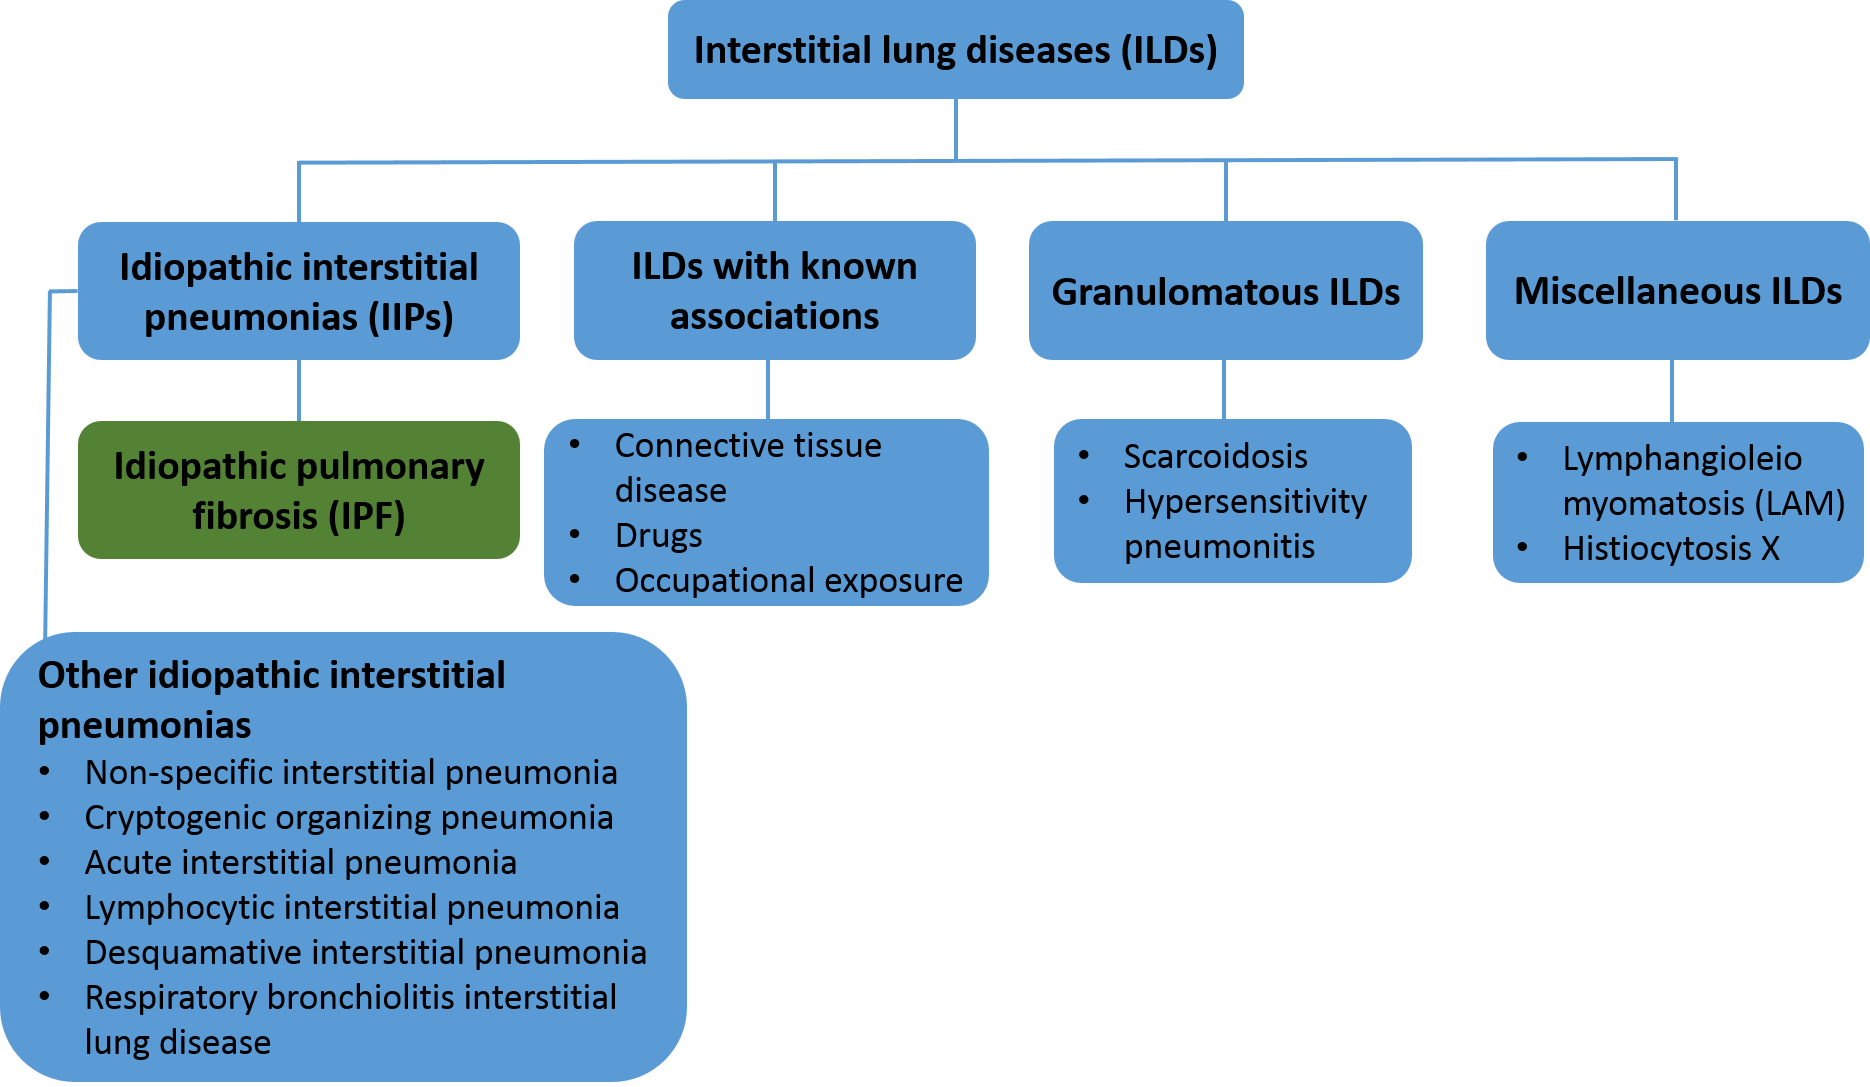
\includegraphics[height=3.5in]{Background/Image/DiseaseClassification.png}
  \caption{Classification of the interstitial lung diseases. IPF belongs to the family of interstitial lung disease (ILD), and belongs to a subgroup known as idiopathic interstitial pneumonia (IIP) \citep{troy2012management}.}
  \label{fig:DiseaseClassification}
\end{figure*}

%%%%%%%%%%%%%%%%%%%%%%%%%%%%%%%%%%%%%%%%%%%%%%%%%%%%%%%%%%%%%%%%%%5
\section{Epidemiology, etiology and pathogenesis} 
\subsection{Epidemiology}
Although IPF is considered a rare disease, this disease is the most common form of IIP \citep{travis2013official}. The incidence of IPF is similar to that of stomach, brain, and testicular cancers and has recently been demonstrated to be rising over time \citep{richeldi2017idiopathic}. A cohort study including patients diagnosed with ILDs at Aarhus University Hospital showed that IPF was the most common diagnosis (28\%) followed by connective tissue disease-related ILD (14\%), hypersensitivity pneumonitis (7\%) and non-specific interstitial pneumonia (NSIP) (7\%) \citep{hyldgaard2014cohort}. Although there is little data available estimating worldwide incidence, a recent study showed that in Europe and North America, the prevalence of IPF is estimated to range between 2.8 and 18 cases per 100,000 people per year, and this value might be lower in Asia and South America, where it is estimated to range from 0.5 to 4.2 cases per 100,000 individuals per year \citep{richeldi2017idiopathic}. IPF is more likely to affect men than women, and is rare in people younger than 50 years \citep{raghu2011official, raghu2006incidence}. The incidence is estimated to be 13 cases/100,000 in women and 20 cases/100,000 in men \citep{xaubet2017idiopathic}. In addition, the incidence of IPF increases with age \citep{meltzer2008idiopathic}. The reason that incidence has increased in recent years is most likely because of improved diagnostic methods and increased life expectancy \citep{xaubet2017idiopathic}.

%%%%%%%%%%%%%%%%%%%%%%%%%%%%%%%%%5
\subsection{Pathogenesis and potential contributors to aetiology}
Historically, IPF was considered a chronic inflammatory disorder, which gradually progressed to established fibrosis \citep{richeldi2017idiopathic}. Now IPF is generally regarded as a consequence of multiple interacting factors, in which repetitive local micro-injuries to an ageing alveolar epithelium plays an important role \citep{richeldi2017idiopathic}. These micro-injuries initiate aberrant epithelial-fibroblast communication, the induction of matrix-producing myofibroblasts, and considerable extracellular matrix accumulation and remodelling of lung interstitium \citep{richeldi2017idiopathic}. Although the aetiology of IPF is unknown, currently,  environmental exposures and genetic factors have been supported by some researchers as providing important inducement \citep{taskar2006idiopathic,meltzer2008idiopathic,xaubet2017idiopathic,richeldi2017idiopathic}. In addition, \gls{ger}, exposure to silica, brass, steel and wood dust, livestock and agriculture work, and the construction of wooden houses are also potential risk factors for the pathogenesis of IPF \citep{taskar2006idiopathic,xaubet2017idiopathic}.

\subsubsection{Environmental exposures}
The relationship between environmental exposures and IPF has been consistently demonstrated by case studies. Asbestosis, for example, is a case in which environmental material is associated with pulmonary fibrosis \citep{meltzer2008idiopathic}. There are studies indicating that the pathogenesis and progression of IPF are influenced by particulate inhalation, which is supported by the fact that the development of IPF consistently relates to cigarette smoking history in most patients \citep{baumgartner1997cigarette,richeldi2017idiopathic}. Additionally, other environmental factors including metal and wood dusts, agriculture and farming, viruses, and stone and silica have also been proposed \citep{raghu2011official, taskar2006idiopathic}.

\newpage

\subsubsection{Genetic factors}
Increasing evidence indicates that genetic predisposition plays an essential part in the development of IPF \citep{xaubet2017idiopathic,richeldi2017idiopathic}. This evidence is based on the existence of familial forms of the disease, and it has been shown that around 2.2\% to 3\% of IPF cases are familial \citep{xaubet2017idiopathic}. The most likely mode of genetic transmission of pulmonary fibrosis in familial cases is autosomal-dominant with variable penetrance \citep{steele2005clinical,allam2006idiopathic,lee2005familial,musk1986genetic}. Rare genetic variants have been identified in cases where ILDs affect two or more members of the same biological family, including genes associated with alterations in host defence (MUC5B, ATP11A, TOLLIP), telomere maintenance (TERT, TERC, PARN, RTEL, OBFC1), surfactant dysfunction (SFTPC, SFTPA2) and epithelial barrier function (DSP, DPP9) \citep{alder2008short,raghu2011official,seibold2011common,xaubet2017idiopathic}. Among them, MUC5B, a promoter site of an airway mucin gene, is the most strongly associated with development of both familial and sporadic IPF \citep{richeldi2017idiopathic}. MUC5B encodes a mucin-5B precursor protein that contributes to airway mucous production and might have an important role in lung host defence. It has also been noted that members of the same biological family may be affected by different types of ILDs, such as non-specific interstitial pneumonia and cryptogenic organizing pneumonia \citep{xaubet2017idiopathic}.

%%%%%%%%%%%%%%%%%%%%%%%%%%%%%%%%%%5
\section{Diagnosis}
The diagnosis of IPF often requires a multidisciplinary discussion, involving pulmonologists, chest radiologists, and chest pathologists experienced in the field of ILDs \citep{flaherty2004idiopathic,king2011idiopathic,raghu2011official}. This multidisciplinary approach has been accepted in consensus guidelines all over the world and has helped to standardize IPF diagnosis \citep{raghu2011official,richeldi2017idiopathic}. Usually, IPF is diagnosed by identification of a pattern of UIP on the basis of radiological or histological criteria in patients without evidence of an alternative cause.  The biggest challenge of diagnosis for clinicians is how to exclude other idiopathic interstitial pneumonias, fibrotic nonspecific interstitial pneumonia, and interstitial lung disease associated with occupational or environmental exposure, connective tissue disease, and drugs \citep{king2011idiopathic,richeldi2017idiopathic}. This differential diagnosis is really important, since typical UIP is not exclusive to IPF, but may associate with some other conditions, such as chronic hypersensitivity pneumonitis and asbestosis. Many patients have a history of environmental exposures or medical treatments which clinicians need to take into consideration for diagnosis \citep{richeldi2017idiopathic}.

\subsection{Clinical presentations}
Patients with IPF usually suffer from unexplained progressive dyspnea on exertion and chronic dry cough, bibasilar inspiratory crackles, and finger clubbing. Bibasilar inspiratory crackles are heard on chest auscultation and finger clubbing is found in about 30\% of patients \citep{raghu2011official,king2011idiopathic,richeldi2017idiopathic}. Chest pain, fatigue, malaise, and weight loss are also typical symptoms for IPF patients \citep{douglas2000idiopathic, king2001predicting}. These clinical presentations might initially be attributed to ageing or some comorbidities such as cardiovascular disease, or obesity \citep{richeldi2017idiopathic}. Therefore, in order to avoid diagnostic delays, it is necessary for primary care physicians to have clinical suspicion of IPF. Some patients may present with acute respiratory exacerbations usually accompanied by fever and influenza-like symptoms within a few days or weeks from the first clinical symptom. In these cases, clinicians require careful diagnostic distinction from other forms of acute ILDs \citep{richeldi2017idiopathic}. Pulmonary function tests (PFTs) from IPF patients usually show a restricted pattern with low percent predicted \gls{tlc} and \gls{dlco}. But for some patients with early disease, PFT results might be normal or mildly abnormal \citep{douglas2000idiopathic,raghu2006incidence}.

\subsection{Radiographic features} \label{RadiographicFeatures}
HRCT of the chest has become an essential tool for the diagnosis of IPF, which is usually associated with identification of a UIP pattern. The presence of UIP pattern on HRCT is characterised by appearance of honeycombing cysts, reticular opacities and ground-glass abnormalities (Figure \ref{fig:RadiologicalImaging}) \citep{king2011idiopathic,raghu2011official,richeldi2017idiopathic}. Honeycombing is common, and essential for a definite diagnosis \citep{raghu2011official}. On HRCT, honeycombing is presented as clustered cystic airspaces with a typical diameter of 3-10 mm but occasionally as large as 2.5 cm, and in a predominantly subpleural and posterior basal distribution \citep{hansell2008fleischner,richeldi2017idiopathic}. Reticular opacities are often associated with traction bronchiectasis \citep{nishimura1992usual, johkoh1999idiopathic}. Ground-glass is a common characteristic of UIP pattern, although it is sometimes less extensive than reticular. The distribution of abnormalities are often basal, peripheral and patchy \citep{raghu2011official}. If patients show micronodules, air-trapping, non-honeycomb cysts, extensive ground glass opacities, consolidation, or a peribronchovascular-predominant distribution, alternative diagnosis should be taken into account \citep{hwang2009computed, souza2006idiopathic}. If patients show reticular abnormalities located in subpleural and basal regions, but no honeycombing appearance, possible UIP patterns should be taken into consideration, then a surgical lung biopsy is suggested to make a definite diagnosis \citep{raghu2011official,richeldi2017idiopathic}. 

\begin{figure}[H]
  \centering 
  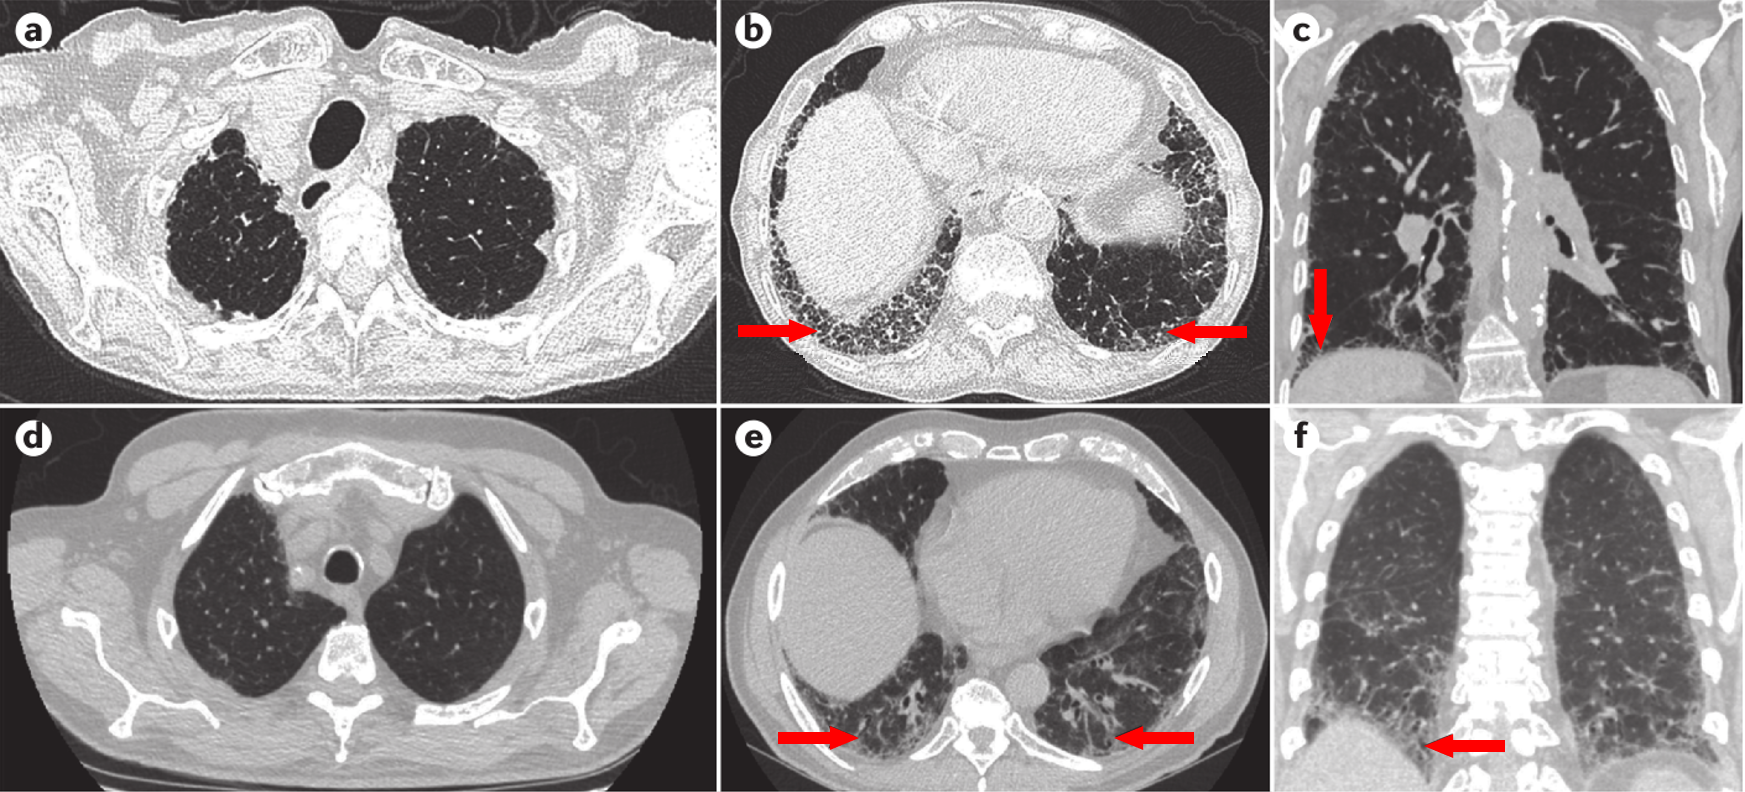
\includegraphics[height=2.5in]{Background/Image/RadiologicalImaging.png}
  \caption{HRCT images of UIP pattern from two patients. The first is from a woman with progressive cough and dyspnoea, showing her upper (a), lower (b) lung zones and a sagittal plane of the lungs (c). These images show lower lobe-predominant peripheral honeycomb change (b and c, arrows), which is typical of UIP pattern. This patient had no systemic disease or exposures that would exclude idiopathic disease: the diagnosis of IPF is certain. In contrast, the second is a woman with progressive breathlessness, who could be diagnosed with possible IPF. The upper (d), lower (e) lung zones and sagittal image of the lungs (f) demonstrate peripheral, basilar-predominant, reticular densities with traction bronchiectasis (e and f, arrows) consistent with fibrosis. Surgical lung biopsy is suggested. Reproduced from \citep{martinez2017idiopathic}.}
  \label{fig:RadiologicalImaging}
\end{figure}


\subsection{Histopathology}
When HRCT features are not enough for a certain diagnosis of IPF, surgical lung biopsy is suggested \citep{richeldi2017idiopathic}. The main histopathologic hallmarks of UIP pattern is characterized by a heterogeneous appearance, best seen at low magnification, with areas of subpleural fibrosis and honeycomb (i.e. cystic fibrotic airspaces lined by bronchiolar epithelium and often filled by mucin and variable numbers of inflammatory cells), alternating with areas of less affected or normal parenchyma \citep{ american2000idiopathic, travis2002american} (Figure \ref{fig:SurgicalLungBiopsy}). Small areas of active fibrosis (fibroblast foci) are present in the background of collagen deposition, and they reflect the temporal heterogeneity and indicate current ongoing disease \citep{king2011idiopathic}. Another feature of UIP pattern is that the inflammation is often absent or mild and consists of a patchy interstitial infiltrate of lymphocytes and plasma cells \citep{raghu2011official,king2011idiopathic}. Although surgical lung biopsy is essential for a correct diagnosis, careful consideration is required for every patient to estimate whether the risks of surgical lung biopsy outweigh the potential benefits of the histopathologic information. For older patients with comorbidities or clinically significant physiological impairment, it is suggested to avoid surgical lung biopsy \citep{richeldi2017idiopathic}.

\begin{figure}[htbp]
  \centering 
  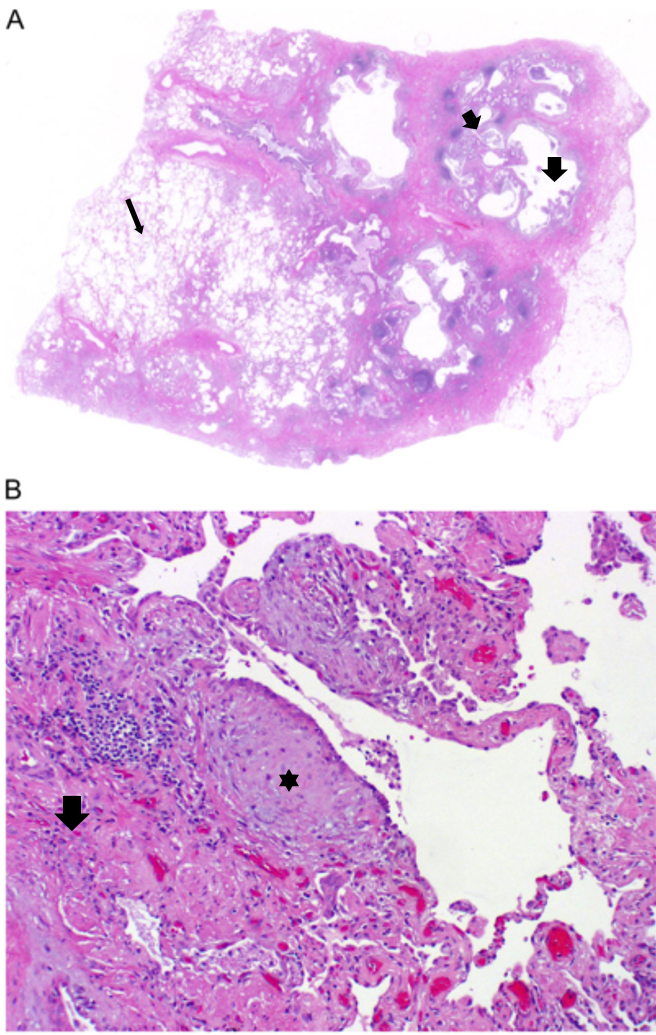
\includegraphics[height=2.9in]{Background/Image/SurgicalLungBiopsy.png}
  \caption{ Surgical lung biopsy specimens of UIP pattern. (A) Scanning power microscopy showing a patchy process with honeycomb
spaces (thick arrow), some preserved lung tissue regions (thin arrow), and fibrosis extending into the lung from the subpleural regions. (B) Adjacent to the regions of more chronic fibrosis (arrow) is a fibroblast focus (asterisk), recognized by its convex shape and composition of edematous fibroblastic tissue, suggestive of recent lung injury. Reproduced from \citep{raghu2011official}.}
  \label{fig:SurgicalLungBiopsy}
\end{figure}

\subsection{Diagnostic criteria} \label{DiagnosisCriteria}
''Gold standard'' diagnostic criteria for IPF have been developed by the \gls{ats} and the \gls{ers} in a statement of published guidelines \citep{raghu2011official}. These criteria are:
\begin{enumerate}
  \item Exclusion of other known causes of ILD (e.g. domestic and occupational environmental exposures, connective tissue disease, and drug toxicity).
  \item The presence of a UIP pattern on HRCT in patients not subjected to surgical lung biopsy.
  \item Specific combinations of HRCT and surgical lung biopsy pattern in patients subjected to surgical lung biopsy.
\end{enumerate}

Beyond that, minor criteria have also been set for the diagnosis of IPF in the absence of a surgical lung biopsy \citep{raghu2011official}:
\begin{enumerate}
  \item Age $>$ 50 years.
	\item Insidious onset of otherwise unexplained dyspnea on exertion.
	\item Duration of illness being over 3 months.
	\item Bibasilar inspiratory crackles (dry or ''Velcro'' type).
\end{enumerate}

Figure \ref{fig:IPFDiagnosis} shows the diagnostic workflow for adult patients with ILD and suspected IPF. If the high-quality HRCT evidence is sufficient enough for the recognition of histopathologic UIP pattern, surgical lung biopsy is not essential \citep{hunninghake2001utility, raghu1999accuracy, flaherty2003radiological, quadrelli2010radiological}. However, a multidisciplinary discussion among experienced clinical, radiologic and histopathologic experts is particularly important when the radiologic and histopathologic patterns are discordant (e.g., HRCT is inconsistent with UIP and histopathology suggests UIP) \citep{raghu2011official}. Radiologic or pathologic UIP pattern is not 100\% specific to IPF \citep{lynch2006usual, trahan2008role, silva2008chronic}.

\begin{figure}[htbp]
  \centering 
  
\includegraphics[height=3.5in]{Background/Image/IPFDiagnosis.png}
  \caption{Diagnostic algorithm for IPF. Patients with suspected IPF (i.e., patients with unexplained dyspnea on exertion and/or cough with evidence of ILD) should be carefully evaluated for identifiable causes of ILD. In the absence of an identifiable cause for ILD, an HRCT demonstrating UIP pattern is diagnostic of IPF. In the absence of UIP pattern on HRCT, IPF can be diagnosed by the combination of specific HRCT and histopathological patterns. The accuracy of the diagnosis of IPF increases with multidisciplinary discussion (MDD) among ILD experts. Reproduced from \citep{raghu2011official}.}
  \label{fig:IPFDiagnosis}
\end{figure}

%%%%%%%%%%%%%%%%%%%%%%%%%%%%%%%%%%%%
\section{Clinical course} 

Some studies indicate that IPF patients have median survival time between two and three years from the time of diagnosis \citep{bjoraker1998prognostic, flaherty2002clinical, nicholson2000prognostic, rudd2007british, king2001idiopathic, king2011idiopathic}. For most IPF patients, the clinical course has been described as a general decline in pulmonary function until eventual death from respiratory failure or complicating comorbidity \citep{carrington1978natural, tukiainen1983prognosis, gross2001idiopathic}, however, the individual disease progression can be highly variable \citep{kim2006classification,meltzer2008idiopathic}. It appears that there are several possible clinical courses for patients with IPF (shown in Figure \ref{fig:IPFDiseaseProgression}) \citep{raghu1987idiopathic}: slow and gradual progression over many years (the most common) \citep{ryu2014idiopathic,meltzer2008idiopathic,raghu2011official}; rapid and accelerated decline \citep{kim2006classification,selman2007accelerated}; and acute exacerbations \citep{king2011idiopathic,xaubet2017idiopathic}. It is difficult to predict the natural history of disease progression for a given patient at the time of the diagnosis \citep{raghu2011official}. Whether the different clinical courses are influenced by geographic, ethnic, cultural, racial, or other factors remains unknown. But some evidence has been suggested that worsening prognosis may be associated with older people ($>$ 70 years old), smoking history, low body mass index (BMI), severe physiological impairment, and large radiological extent of disease \citep{ley2011clinical}. Other comorbidities such as emphysema and pulmonary hypertension may also have an impact on the disease course \citep{mejia2009idiopathic, wells2003idiopathic, lettieri2006prevalence}. While prediction of the likely course of disease is currently not possible, it would be very beneficial to enable clinicians to make an appropriate and optimal treatment plan as early as possible.
\newpage

\subsection{Slow and rapid progressive course}
Most IPF patients deteriorate relatively slowly, and their pulmonary function usually decreases gradually over months to years after the first clinical symptoms (cough and progressive dyspnoea) \citep{ryu2014idiopathic,meltzer2008idiopathic,raghu2011official}. Patients usually experience reduction of lung volumes, and hypoxaemia at rest that worsens with exercise. This is accompanied by a decline of \gls{fvc}  by a mean of 0.13 L to 0.21 L per year \citep{ley2011clinical}. In contrast, a subgroup of patients with IPF, mainly male cigarette smokers, experience a rapid worsening of symptoms, and insufficiency of pulmonary function \citep{kim2006classification, king2011idiopathic}, known as accelerated IPF. The patients with rapid progression have reduced survival time relative to those with a slowly progressive clinical course.

\subsection{Acute exacerbations of IPF}
“Acute exacerbation” was first proposed by Japanese physicians to describe acute, unexpected worsening of respiratory functions and severe hypoxaemia in patients with IPF, without a clear trigger \citep{kondoh1993acute, gross1962concept}. The rapid deterioration occurs in a small minority of patients with IPF (about 5-10\%), with absence of infection, heart failure, pneumothorax, or pulmonary embolism \citep{azuma2005double,king2011idiopathic,raghu2011official}. The prognosis for patients with acute exacerbations is poor, and it may happen at any stage in the course of IPF \citep{kim2006acute,parambil2005histopathologic,sakamoto2009acute,kondoh2010prognostic}. Patients with acute exacerbation usually experience poor respiratory decline, worsened cough, fever and increased sputum production \citep{ambrosini2003acute,kim2006acute}. The mortality rate for patients with acute exacerbations is over 60\% \citep{wootton2011viral, lettieri2006prevalence}; for cases requiring mechanical ventilation, the mortality is close to 100\% \citep{king2011idiopathic,xaubet2017idiopathic}.

\begin{figure}[htbp]
  \centering 
  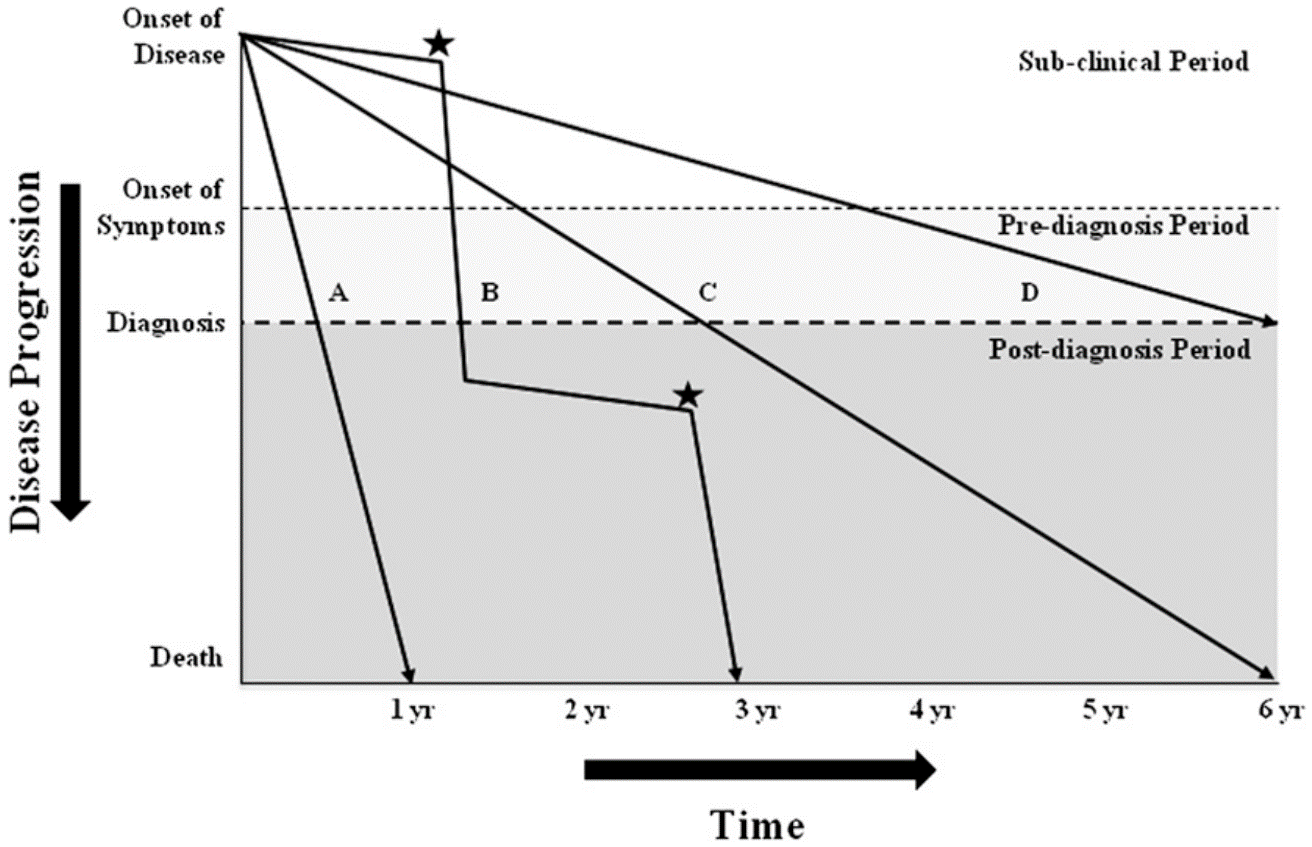
\includegraphics[height=3.2in]{Background/Image/IPFDiseaseProgression.png}
  \caption{Schematic representation of potential clinical courses of IPF.  A sub-clinical period of disease progression exists during which only radiographic evidence of disease may be noted. This is followed by a symptomatic phase comprising clinical stages (both pre-diagnosis and post-diagnosis). The rate of deterioration and progression to death may be fast (line A), mixed (line B), or slow (lines C and D), with phases of relative disease stability interspersed with acute decline (asterisks). Reproduced from \citep{ley2011clinical}.}
  \label{fig:IPFDiseaseProgression}
\end{figure}

%%%%%%%%%%%%%%%%%%%%%%%%%%%%%%%%%%%5
\section{Complications and comorbidities}
%For the purposes of diagnoses, a complication is a condition that arises during the hospital stay, and a comorbidity is a pre-existing condition that affects the treatment received. 
Complications and comorbidities can occur in patients with IPF that may influence the clinical course and prognosis \citep{xaubet2017idiopathic,king2017idiopathic,martinez2017idiopathic}. It is reported that only 12\% of patients with IPF have no comorbid illness, and most patients have comorbidities \citep{raghu2011official, kim2015natural, harari2016epidemiology, kreuter2016impact}. Emphysema and pulmonary hypertension are both important comorbid conditions in IPF patients \citep{raghu2015comorbidities,martinez2017idiopathic}, and are briefly outlined here.

\subsection{IPF and emphysema}

Several research groups have described a syndrome in which IPF coexists with pulmonary emphysema \citep{wells1997lone, wells2003idiopathic, cottin2005combined,meltzer2008idiopathic}. In 2005, \cite{cottin2005combined} presented a syndrome named \gls{cpfe}. Both IPF and emphysema are associated with a significant smoking history, and CPFE is strongly associated with exercise hypoxaemia, severe dyspnea on exertion, upper lobe emphysema and lower lobe fibrosis, unexpected subnormal lung volumes, and severe reduction of carbon monoxide transfer \citep{silva2008idiopathic,mejia2009idiopathic,cottin2010pulmonary,king2011idiopathic,lin2015combined}. Currently, whether CPFE is a distinct clinical entity or not remains unknown, i.e. whether this is just the presence of two different diseases running in parallel is unclear \citep{king2011idiopathic,lin2015combined}. Some researchers suggest that CPFE should be regarded as a distinct clinical entity, since it has a characteristic pulmonary function feature and unique natural history that is different from pure emphysema or IPF alone \citep{cottin2005combined, lin2015combined, xaubet2017idiopathic}. CPFE occurs more frequently in males than in females and its prevalence is about 30\% to 47\% in patients with IPF \citep{xaubet2017idiopathic}. It is often associated with a significant drop of DLCO and severe hypoxaemia during exercise due to the additive effect of emphysema and fibrosis \citep{xaubet2017idiopathic}. 
\newpage

\begin{figure}[htbp]
  \centering 
  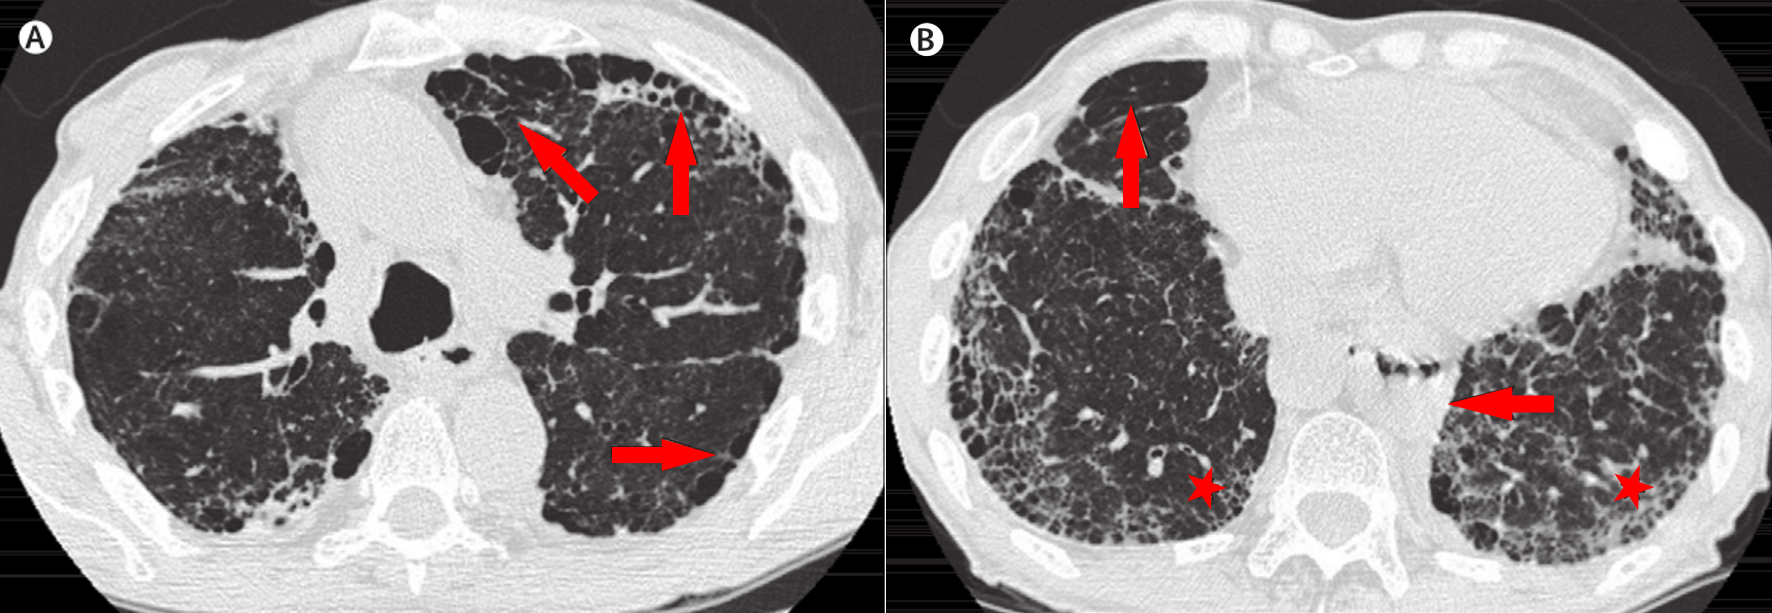
\includegraphics[height=2.05in]{Background/Image/CPFEImaging.png}
  \caption{ Combined pulmonary fibrosis and emphysema. High-resolution CT shows emphysematous lesions (arrows) in the upper lobes (in Figure A), emphysema (arrow) and usual interstitial pneumonia-like lesions (stars) in the lower lobes (in Figure B). Reproduced from \citep{king2011idiopathic}.}
  \label{fig:CPFEImaging}
\end{figure}

\subsection{IPF and pulmonary hypertension}
Pulmonary hypertension (PH), defined as a mean pulmonary artery pressure of $>$ 25 mmHg at rest, is a frequent form of comorbid condition in patients with IPF and is the main determinant of poor prognosis \citep{raghu2011official, xaubet2017idiopathic}. It is estimated that the incidence of pulmonary hypertension is around 30\% to 50\% in IPF patients \citep{king2017idiopathic}. In general, pulmonary hypertension occurs due to several factors, with chronic hypoxia-induced vasoconstriction and destruction of the pulmonary capillary bed induced by fibrosis being the two main causes \citep{hayes2016influence}. The presence and development of pulmonary hypertension is associated with significant dyspnea, functional impairment (particularly in DLCO) and decreased exercise capacity, and may increase risk of mortality for patients with IPF \citep{mejia2009idiopathic,lettieri2006prevalence,nadrous2005impact}. Some studies have shown that combined pulmonary fibrosis and pulmonary hypertension has a significantly negative effect on the survival in patients with IPF alone, probably caused by the increased pulmonary vascular resistance \citep{raghu2011official, king2011idiopathic}. Currently, whether IPF with pulmonary hypertension represents a distinct  clinical entity (IPF–PH) is still unclear \citep{raghu2011official}.

%%%%%%%%%%%%%%%%%%%%%%%%%%%%%%%%%%%%%%%%%5
\section{Physiological alterations}
The clinical presentation of IPF is related to a number of physiological alterations of the lung \citep{crystal1976idiopathic, plantier2018physiology}. These alterations have a complex and negative impact on all compartments of the respiratory system, from lung volume and compliance to gas exchange, from conducting airways to lung vasculature \citep{plantier2018physiology}. In general, patients with IPF usually have reduced lung volumes, reduced lung compliance, reduced diffusing capacity, increased \gls{fev1/fvc}, and arterial hypoxaemia that worsens with exercise \citep{crystal1976idiopathic,american2000idiopathic,cortes2014idiopathic,plantier2018physiology}. These alterations in lung physiology are summarized in Table \ref{tab:IPFPhysiologicAlterations}.

\begin{table}[htbp]
\centering
\caption{Alterations of lung function tests in \gls{ipf} Reproduced from \citep{plantier2018physiology}}
\label{tab:IPFPhysiologicAlterations}
\begin{tabular}{l c c}
\hline
  & \bf{Mild IPF} & \bf{Moderate to severe IPF} \\ 
\hline
\bf{Static lung volumes} &  &  \\
- TLC & Normal & Decreased\\
- FRC & Normal & Decreased\\
\hline
\bf{Spirometry} &  &  \\
- FVC & Normal & Decreased\\
- FE$V_1$/FVC & Normal or increased & Normal or increased\\
\hline
\bf{Airways} &  &  \\
- Cough reflex & Increased & Increased\\
- Airway resistance & Decreased & Decreased\\
\hline
\bf{Blood gases at rest} &  &  \\
- $P_aO_2$ & Normal & Decreased\\
- $P_aCO_2$ & Normal & Decreased\\
\hline
\bf{Carbon monoxide transfer} &  &  \\
- DLCO & Decreased & Decreased\\
- $V_A$ & May be normal & Decreased\\
- $K_{CO}$ & May be normal & Decreased\\
\hline
\bf{Exercise physiology} &  &  \\
- Peak $V_{O_2}$ & May be normal & Decreased\\
- $V_D/V_T$ & Increased & Increased\\
- $V_E/V_{CO_2}$ & Increased & Increased\\
- PAP at exercise & Increased & Increased\\
- $P_{A-a} O_2$ at exercise & Increased & Increased\\
\hline
\bf{Pulmonary haemodynamics at rest} &  &  \\
- PAP & May be increased & Frequently increased\\
- PCWP & Normal & May be increased\\
\hline
\end{tabular}
\begin{tablenotes}
        \footnotesize
        \item{FVC: forced vital capacity; FE$V_1$ : forced expiratory volume in 1 s; TLC: total lung capacity; FRC: functional residual capacity; $P_aO_2$ : arterial oxygen tension; $P_aCO_2$ : arterial carbon dioxide tension; DLCO : diffusing capacity of the lung for carbon monoxide; $V_A$ : alveolar volume; $K_CO$ : transfer constant of carbon monoxide; PAP: pulmonary artery pressure; PCWP: pulmonary capillary wedge pressure; $V_{O_2}$ : oxygen uptake; $V_D/V_T$ : ratio of dead space volume to tidal volume; $V_E/V_{CO_2}$ : ratio of minute ventilation to carbon dioxide elimination; $P_{A-a} O_2$ : alveolar–arterial oxygen tension difference.}
\end{tablenotes}
\end{table}

\subsection{Alterations in the mechanical properties of the lung} \label{MechanicalAlteration}
\subsubsection{Reduction in lung compliance}
IPF disease often results in reduction in lung compliance (i.e. an increase in lung tissue stiffness). Studies have shown that the reduced lung compliance is caused by a reduction in the compliance of the lung extracellular matrix and by alterations in pulmonary surfactant \citep{plantier2018physiology}. In patients with IPF, surfactant shows alterations in its lipid profile \citep{gunther1999surfactant, schmidt2002altered}, which leads to severely impaired surface activity \citep{gunther1999surfactant}. The reduction in lung compliance may happen from an early stage of IPF \citep{plantier2018physiology}. A study of 31 IPF patients from \citep{zielonka2010angiogenic} showed that the static lung compliance was consistently and significantly reduced (by 44 $\pm$ 6\%). A similar result was found by in another study \citep{orens1995sensitivity}, where all of the measured IPF patients had abnormal static lung compliance, which suggests that measurement of lung compliance could help with the early diagnosis of IPF.

The alterations of lung compliance in IPF patients appear to be strongly correlated with the degree of lung fibrosis as assessed by scoring of lung biopsies \citep{fulmer1979morphologic,plantier2018physiology}. \cite{nava1999lung} measured the dynamic lung compliance in seven patients with end-stage IPF, which showed that the reduction in lung compliance may be correlated with the progress of the disease. Currently, whether the reductions in lung compliance relate to clinical presentations (e.g. dyspnoea) remains unclear, but it is highly likely that the lung compliance has a strong relationship with the respiratory muscles and thus has an impact on the work of breathing \citep{plantier2018physiology}. In addition, as the distribution of disease is heterogeneous in IPF lungs, lung compliance is expected to be uneven between different lung regions \citep{organ2015structural}, but more evidence is needed to understand the implications of disease distribution outcomes.

\subsubsection{Reduction of lung volumes}
The restriction of lung volumes (total lung capacity (TLC), \gls{frc}, forced vital capacity (FVC), and \gls{rv}) is typical in patients with IPF. This restriction of lung volumes often occurs at some time point in the clinical course of IPF \citep{american2000idiopathic, plantier2018physiology}. However, sometimes lung volumes may be normal in the early stage of IPF, especially for patients with superimposed chronic obstructive pulmonary disease \citep{martinez2006pulmonary}. \cite{cherniack1995correlation} studied 96 patients with biopsy-confirmed IPF. The range of TLC was from 42\% to 125\% predicted and the range of FVC was from 26\% to 112\% predicted. A reduction in lung volumes consistently relates to an increased risk of death \citep{martinez2006pulmonary}, and is weakly associated with dyspnoea or quality of life \citep{du2011ascertainment}. However, whether the reduced lung volumes reflects the disease progression of IPF is still unknown \citep{plantier2018physiology}. Interestingly, patients with CPFE have higher RV and TLC compared to the patients with IPF alone \citep{mura2006presence}, which may be caused by the effects of comorbid pulmonary emphysema on lung compliance \citep{doherty1997cryptogenic}.

\subsubsection{Alterations in the conducting airways}
Some evidence suggests that alterations also occur in conducting airways in patients with IPF, including increased airway epithelial cell proliferation \citep{vuorinen2008peroxiredoxin} and differentiation \citep{plantier2016increased}, and increased numbers of visible bronchioles in the distal regions \citep{chilosi2002abnormal}. A reduction in conducting airway resistance was found in IPF lungs compared with normal, which may contribute to an increased ratio of FE$V_1$ to FVC \citep{pastre2015different}. \cite{plantier2016increased} used volumetric capnography to estimate the volume of conducting airways in patients with IPF, patients with other ILDs, and healthy people. The results showed that conducting airway volume was significantly higher in IPF lungs in comparison with non-IPF ILD lungs and healthy lungs. However, this change in airway volume was not associated with the severity of alveolar lesions, dyspnea, cough or quality of life \citep{plantier2016increased}. The increase in airway volume in IPF may reflect dilation of airways consistent with bronchiectasis that can be characteristic of this disease, and a commonly accepted view is that bronchiectasis in IPF may be caused by fibrotic retraction of peribronchiolar alveolar attachments and subsequent airway dilation \citep{sumikawa2008computed}. However, a recent study found that bronchiectasis had a weak relationship with total fibrosis extent observed from CT imaging \citep{walsh2015relationship}, which means the remodelling of conducting airways in IPF may be dissociated from alveolar fibrosis \citep{plantier2016increased}. Patients with IPF usually have more rapid breaths with the progression of disease \citep{kornbluth1980respiratory, renzi1982pattern}, and have a relatively increased flow rate in the conducting airways due to the increased static elastic recoil \citep{american2000idiopathic}. Additionally, it has been suggested that at least part of the ventilation abnormalities seen in IPF is associated with small airways disease with peribronchiolar fibrosis and inflammation, and 70\% of IPF patients have narrowed small airways \citep{crystal1976idiopathic}.

\subsubsection{Alterations in the lung vasculature} \label{VasculatureAlterations}
Vascular lesions are observed in the pulmonary vasculature in patients with IPF, and often lead to disproportionate increases in the pulmonary vascular resistance and pulmonary hypertension \citep{plantier2018physiology}. The tissues adjacent to the areas of fibrosis have been shown to have an increase in vessel profusion, whereas the fibrotic tissue itself demonstrates a reduced number of blood vessels \citep{cosgrove2004pigment,ebina2004heterogeneous}. \cite{Jacob2016Evaluation} explored the relationship between \gls{pvv} and ILD extent (includes ground glass, reticular and honeycomb patterns). It was found that PVV had a strong relationship with ILD extent ($R^2 = 0.73$, $P < 0.0001$) when using linear regression analysis. Furthermore, PVV was demonstrated to be an independent predictor of mortality, and a stronger predictor of mortality than all the other traditional CT features and pulmonary functional variables \citep{Jacob2016Evaluation}. The increase in PVV seen in more advanced fibrosis may be caused by the vascular capacitance of spared lung (the upper and middle lobes in patients with IPF, which is a predominantly basal disease), and may also relate to the increased negative intrathoracic pressure which non-compliant fibrotic lungs need to generate during inspiration \citep{Jacob2016Mortality}.

\subsection{Alterations in pulmonary gas exchange}
IPF is associated with multiple pathophysiological changes in pulmonary gas exchange. The lesions of the alveolar-capillary membrane in IPF lungs will impair both the diffusion capacity and ventilation/perfusion (V/Q) relationship, increase dead space ventilation and alveolar-arterial oxygen tension difference ($P_{A-a}O_2$), and finally cause chronic arterial hypoxaemia \citep{crystal1976idiopathic,plantier2018physiology,american2000idiopathic}.

\subsubsection{Reduced diffusing capacity of the lung}
The diffusing capacity of oxygen is considered to be reduced in almost all patients with IPF. However, in clinical examination, this diffusing capacity is technically very difficult to measure. Therefore, clinical tests actually measure the diffusing capacity of carbon monoxide (DLCO) which provides an estimate of the gas-exchange function of the whole lungs \citep{plantier2018physiology}. DLCO is a measure of the conductance of gas transfer from inspired gas to the red blood cells, and is usually tested in a single breath where the partial pressure difference between inspired and expired carbon monoxide is recorded \citep{rosenberg19961995,plantier2018physiology}. The \gls{kco} is an index of the efficiency of alveolar transfer of carbon monoxide. It can be referred to as DLCO/VA, where VA is the alveolar volume where gas exchange takes place \citep{graham20172017}.

It has been shown that DLCO is reduced compared with normal values in 98\% of IPF patients at initial diagnosis, although 27\% of patients have normal TLC volumes, and 56\% have normal FVC \citep{cortes2014idiopathic}. Interestingly, KCO is within the normal range in up to 30\% of IPF patients \citep{wallaert2012we}, particularly in patients with moderately reduced DLCO \citep{pastre2015different}. But a normal KCO value in IPF patients does not mean that pulmonary gas exchange is normal \citep{plantier2018physiology}. It has been noted that both DLCO and KCO are significantly associated with the degree of IPF measured from CT scans \citep{wells1997lone}, but DLCO correlates more strongly with exertional increases in $P_{A-a}O_2$ \citep{agusti1994clinical} and highly relates to both dyspnoea \citep{swigris2012ucsd} and survival time \citep{hamada2007significance}.

\subsubsection{Dead space ventilation}
Increased physiologic dead space ventilation (increased ratio of dead space volume to tidal volume $\mathrm{V_D}/V_T$) is an important characteristic of lungs with fibrosis and happens in most IPF patients both at rest and at exercise \citep{fulmer1976diffuse, crystal1976idiopathic, agusti1991mechanisms, miki2009acidosis}. The increased dead space is mainly caused by two physiologic features: the first is the increased anatomical dead space, which is a result of the dilation of conducting airways in IPF as discussed in Section \ref{MechanicalAlteration} \citep{plantier2016increased}; the second is the regional ventilation-perfusion mismatch (increased variation in regional ventilation-perfusion ratio, V/Q), which increases the physiologic dead space. In IPF lungs, the fibrotic (i.e. honeycomb or reticular) areas that are  not perfused or poorly perfused but still receive ventilation will have an increased regional V/Q ratio \citep{strickland1993cause, plantier2018physiology}. An early paper indicated that patients with IPF will often have a $\mathrm{V_D}/V_T$ ratio of greater than 0.4 compared with a normal person (approximate 0.3 for normal) \citep{crystal1976idiopathic}. In normal individuals the efficiency of ventilation improves with exercise (that is the VD/VT falls) \citep{ jones1966physiological, wasserman1975exercise}, but in more than 90\% of IPF patients $\mathrm{V_D}/V_T$ stays constant or may increase \citep{crystal1976idiopathic}. 

\subsubsection{Ventilation-perfusion mismatching}

It is generally thought that the hypoxemia of IPF is related to V/Q mismatching \citep{wagner1976distribution,crystal1976idiopathic,american2000idiopathic}. This V/Q mismatching may be associated with abnormalities both in ventilation and perfusion \citep{crystal1976idiopathic,strickland1993cause}. \cite{crystal1976idiopathic} showed an equilibrium picture of 127 Xe distribution, which was used to determine regional ventilation, and showed that patients with IPF have patchy, non-segmental areas of decreased ventilation where airway obstruction or alveolar destruction occurred. As for perfusion, a shift of perfusion was observed to the upper lobes (reflecting pulmonary hypertension) due to the basal distribution of fibrotic lesions, so that areas of relatively low V/Q ratios mostly presented in the upper zones of the lung \citep{crystal1976idiopathic}. However, \cite{strickland1993cause} indicated that the CT based cystic air spaces (i.e. honeycomb) were observed as poorly perfused (probably due to vascular obliteration) but were usually  normally ventilated, which explains the increase in physiologic dead space seen at rest and with exercise. Thus, a higher V/Q ratio can be seen in areas where fibrosis and cystic air spaces are dominant, which could be used to distinguish IPF from emphysema \citep{strickland1993cause}. In addition, an increased minute ventilation was found in most patients with IPF during exercise. This is mainly due to the increased respiratory frequency, and in part relates to an increase in dead space ventilation \citep{american2000idiopathic}.

\subsubsection{Arterial hypoxaemia}
Alterations in the mechanical properties of the lungs, impairment of diffusion capacity and ventilation-perfusion mismatch will finally lead to early-onset exertional chronic arterial hypoxaemia and later-onset resting chronic arterial hypoxaemia in IPF \citep{hempleman1991estimating, hughes1991dlco, plantier2018physiology}. Some studies support that the major cause of arterial hypoxaemia in a large proportion of IPF patients is not the diffusion barrier to oxygen or the anatomic shunts, as was originally suspected, but is due to ventilation-perfusion mismatching \citep{ finley1962cause, wagner1976distribution, american2000idiopathic}. The alveolar-arterial oxygen gradient ($P_{A-a}O_2$), which is calculated from arterial oxygen tension ($P_{a}O_2$) and alveolar oxygen tension ($P_{A}O_2$) may increase, resulting from the reduced ventilation-perfusion ratio, right-to-left shunting, or impairment of oxygen diffusion \citep{plantier2018physiology}. The increase in $P_{A-a}O_2$ reflects hypoxaemia in IPF \citep{agusti1991mechanisms}. In a study of 29 IPF patients, the measured average resting $P_a O_2$ was 69.3 mmHg, and four patients had normal resting $P_{a}O_2$. However, although the resting $P_{a}O_2$ can be normal in some IPF patients, the resting $P_{A-a}O_2$ is invariably abnormal (in about 97\% of the patients with IPF) \citep{crystal1976idiopathic}.

%%%%%%%%%%%%%%%%%%%%%%%%%%%%%%%%5
\section{Summary}
IPF is a devastating lung disease characterized by an irreversible decline of lung function, and its incidence increases with years of age. The current efforts of studies in IPF mostly focus on the  accurate identification and diagnosis of early IPF, underlying mechanisms of pathogenesis and potential bio-markers that can indicate the patient-specific clinical course. The presence of IPF is variable in most patients, but some common characteristics and progressions can be summarized, although this is challenging. The clinical and physiological features of IPF reviewed in this chapter provides background information for further quantitative analysis (Chapter 4) and computational modelling of patients with IPF (Chapter 5). 
